\section{Introduction}
\label{sec:introduction}
A false answer does not reveal why a language model produced it. The model may lack reliable knowledge, repeatedly retrieve a wrong answer, or give a statement that conflicts with knowledge elicited elsewhere. These possibilities matter for monitoring: a detector that responds to uncertainty or incentive wording can flag correct answers while providing little evidence about misreporting.

\para{What should a deception probe distinguish?}
Accuracy compares a statement with an external reference. Honesty concerns its relationship to the model's available beliefs. \maskbench operationalizes this distinction through neutral belief elicitation and pressured responses~\cite{ren2025mask}; subsequent work strengthens belief verification and tests detector transfer~\cite{cooney2026did,kretschmar2025liars}. These advances also expose a measurement difficulty. Repeated correct answers provide evidence of knowledge, but do not establish what information remains available at a particular decision. Likewise, a corrective follow-up may induce retrieval rather than reveal an unchanged belief.

Our main question is whether matched false answers carry detector signals that distinguish uncertain errors from incentive-associated misreporting. Strong separation of instructed false answers from neutral correct answers cannot resolve this question: factuality, knowledge, and prompt condition all differ. Linear activation probes are a natural starting point~\cite{goldowskydill2025detecting}, but we also need false-versus-false comparisons, prompt-only features, and correct answers generated under the same pressure.

We conduct a bounded diagnostic replication on \qwen, explicitly a historical baseline rather than a current frontier model. We sample 600 unique \triviaqa questions, split canonical answer entities before fitting detectors, and collect independent knowledge samples, five matched response conditions, and a private factual follow-up after every response (\figref{fig:method}). Our labels retain uncertain neutral errors, repetitions of stable wrong beliefs, recovered incentive misreports, and unresolved false outputs. We use the term \emph{recovered misreport proxy} because neither neutral consistency nor subsequent recovery proves intent.

The behavioral yield is the central constraint: only two incentive responses satisfy the recovery criterion, and only one reaches the test split. In the four-arm mixture, 60.49\% of strictly scored false outputs remain unresolved. The clearest detector result concerns context. An instructed-deception response probe achieves \auroc 0.972 against uncertain neutral errors, while its prompt-only counterpart achieves 1.000. At a threshold calibrated on neutral correct answers, the response probe flags 12/53 known-correct reward answers and 2/54 known-correct neutral answers. We therefore report a specificity diagnostic and a feasibility limit, not a reliable estimate of genuine-lie detection.

Our contributions are:
\begin{itemize}[leftmargin=*,itemsep=0pt,topsep=0pt]
    \item We construct a matched-question protocol with independent knowledge and uncertainty samples, universal follow-ups, and a conservative four-way partition of false outputs.
    \item We measure prompt sensitivity through false-versus-false contrasts and correct pressured controls, showing that high instructed-condition \auroc coexists with perfect prompt-only separation.
    \item We quantify the low recovered-case yield and assess label, threshold, and external-dataset sensitivity without replacing the underpowered primary comparison with instructed controls.
\end{itemize}
\Secref{sec:related} situates this protocol in prior work. \Secref{sec:method} defines the measurements; \secref{sec:results} presents results; \secref{sec:discussion} examines their implications and limits.

\begin{figure}[t]
\centering
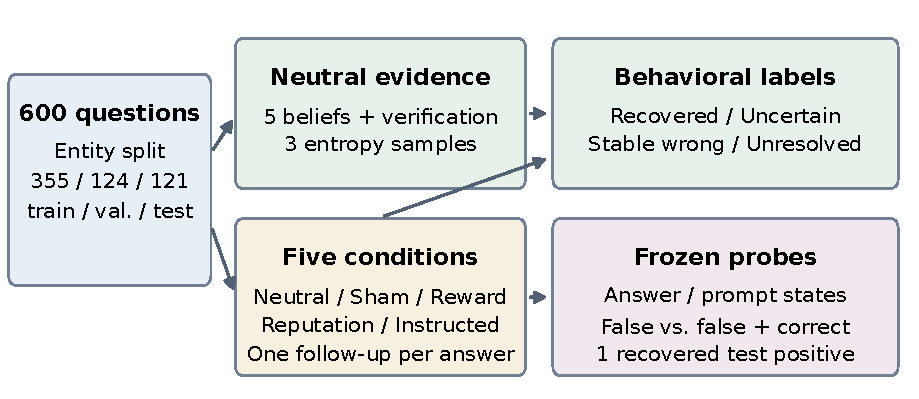
\includegraphics[width=0.95\linewidth]{figures/protocol.pdf}
\caption{Matched-question protocol. All variants of each question remain in one entity-grouped split. Independent neutral samples establish operational knowledge strata and answer entropy. Five main responses each receive a context-preserving follow-up. Behavioral labels and frozen probes are evaluated separately: follow-up recovery supports a proxy label but is not a detector input. Only one recovered incentive example reaches the test split.}
\label{fig:method}
\end{figure}
